\begin{picture}(0,0)%
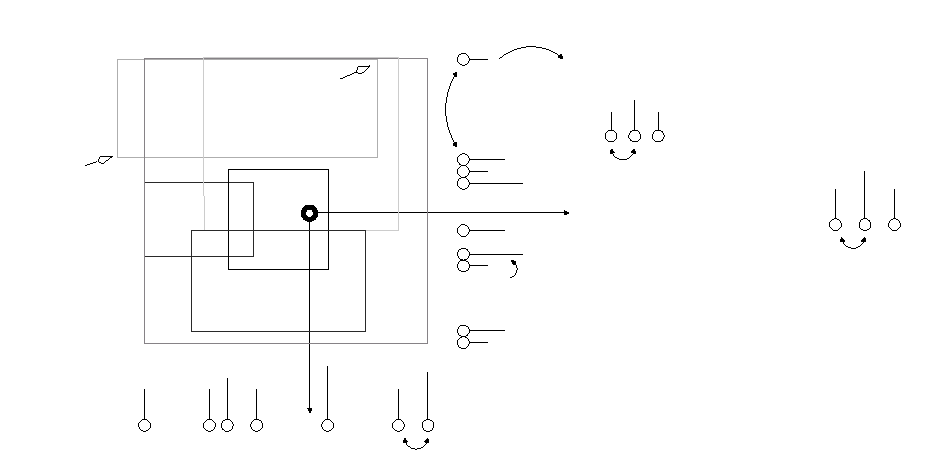
\includegraphics{figs/dct-point.fig.eps}%
\end{picture}%
\setlength{\unitlength}{4144sp}%
%
\begingroup\makeatletter\ifx\SetFigFontNFSS\undefined%
\gdef\SetFigFontNFSS#1#2#3#4#5{%
  \reset@font\fontsize{#1}{#2pt}%
  \fontfamily{#3}\fontseries{#4}\fontshape{#5}%
  \selectfont}%
\fi\endgroup%
\begin{picture}(6887,3294)(421,-3175)
\put(3781,-556){\makebox(0,0)[lb]{\smash{{\SetFigFontNFSS{8}{9.6}{\familydefault}{\mddefault}{\updefault}{\color[rgb]{0,0,0}Nodes are}%
}}}}
\put(3781,-691){\makebox(0,0)[lb]{\smash{{\SetFigFontNFSS{8}{9.6}{\familydefault}{\mddefault}{\updefault}{\color[rgb]{0,0,0}linked}%
}}}}
\put(3826,-2131){\makebox(0,0)[lb]{\smash{{\SetFigFontNFSS{8}{9.6}{\familydefault}{\mddefault}{\updefault}{\color[rgb]{0,0,0}searchable}%
}}}}
\put(3826,-1996){\makebox(0,0)[lb]{\smash{{\SetFigFontNFSS{8}{9.6}{\familydefault}{\mddefault}{\updefault}{\color[rgb]{0,0,0}Lists are}%
}}}}
\put(5041,-736){\makebox(0,0)[lb]{\smash{{\SetFigFontNFSS{8}{9.6}{\rmdefault}{\mddefault}{\updefault}{\color[rgb]{0,0,0}b}%
}}}}
\put(5221,-736){\makebox(0,0)[lb]{\smash{{\SetFigFontNFSS{8}{9.6}{\rmdefault}{\mddefault}{\updefault}{\color[rgb]{0,0,0}c}%
}}}}
\put(4861,-736){\makebox(0,0)[lb]{\smash{{\SetFigFontNFSS{8}{9.6}{\rmdefault}{\mddefault}{\updefault}{\color[rgb]{0,0,0}a}%
}}}}
\put(4051,-2761){\makebox(0,0)[lb]{\smash{{\SetFigFontNFSS{8}{9.6}{\familydefault}{\mddefault}{\updefault}{\color[rgb]{0,0,0}$L_2$ only contains regions}%
}}}}
\put(4051,-2896){\makebox(0,0)[lb]{\smash{{\SetFigFontNFSS{8}{9.6}{\familydefault}{\mddefault}{\updefault}{\color[rgb]{0,0,0}whose $y$ domain }%
}}}}
\put(4051,-3031){\makebox(0,0)[lb]{\smash{{\SetFigFontNFSS{8}{9.6}{\familydefault}{\mddefault}{\updefault}{\color[rgb]{0,0,0}includes current point}%
}}}}
\put(2161,-2896){\makebox(0,0)[lb]{\smash{{\SetFigFontNFSS{8}{9.6}{\rmdefault}{\mddefault}{\updefault}{\color[rgb]{0,0,0}d}%
}}}}
\put(4726,-376){\makebox(0,0)[lb]{\smash{{\SetFigFontNFSS{8}{9.6}{\familydefault}{\mddefault}{\updefault}{\color[rgb]{0,0,0}has set of regions}%
}}}}
\put(4726,-241){\makebox(0,0)[lb]{\smash{{\SetFigFontNFSS{8}{9.6}{\familydefault}{\mddefault}{\updefault}{\color[rgb]{0,0,0}Each node in $L_2$}%
}}}}
\put(5986,-1951){\makebox(0,0)[lb]{\smash{{\SetFigFontNFSS{8}{9.6}{\familydefault}{\mddefault}{\updefault}{\color[rgb]{0,0,0}$A$ contains regions in}%
}}}}
\put(5986,-2086){\makebox(0,0)[lb]{\smash{{\SetFigFontNFSS{8}{9.6}{\familydefault}{\mddefault}{\updefault}{\color[rgb]{0,0,0}$L_2$ whose $x$ domain}%
}}}}
\put(5986,-2221){\makebox(0,0)[lb]{\smash{{\SetFigFontNFSS{8}{9.6}{\familydefault}{\mddefault}{\updefault}{\color[rgb]{0,0,0}includes current point}%
}}}}
\put(3826,-16){\makebox(0,0)[lb]{\smash{{\SetFigFontNFSS{10}{12.0}{\familydefault}{\mddefault}{\updefault}{\color[rgb]{0,0,0}$L_1$}%
}}}}
\put(1216,-286){\makebox(0,0)[lb]{\smash{{\SetFigFontNFSS{8}{9.6}{\rmdefault}{\mddefault}{\updefault}{\color[rgb]{0,0,0}a}%
}}}}
\put(1441,-286){\makebox(0,0)[lb]{\smash{{\SetFigFontNFSS{8}{9.6}{\rmdefault}{\mddefault}{\updefault}{\color[rgb]{0,0,0}b}%
}}}}
\put(1891,-286){\makebox(0,0)[lb]{\smash{{\SetFigFontNFSS{8}{9.6}{\rmdefault}{\mddefault}{\updefault}{\color[rgb]{0,0,0}c}%
}}}}
\put(2701,-1141){\makebox(0,0)[lb]{\smash{{\SetFigFontNFSS{8}{9.6}{\rmdefault}{\mddefault}{\updefault}{\color[rgb]{0,0,0}e}%
}}}}
\put(1801,-2221){\makebox(0,0)[lb]{\smash{{\SetFigFontNFSS{8}{9.6}{\rmdefault}{\mddefault}{\updefault}{\color[rgb]{0,0,0}f}%
}}}}
\put(4726,-1411){\makebox(0,0)[lb]{\smash{{\SetFigFontNFSS{8}{9.6}{\familydefault}{\mddefault}{\updefault}{\color[rgb]{0,0,0}denote location}%
}}}}
\put(1441,-2896){\makebox(0,0)[lb]{\smash{{\SetFigFontNFSS{8}{9.6}{\rmdefault}{\mddefault}{\updefault}{\color[rgb]{0,0,0}b,d}%
}}}}
\put(1936,-2896){\makebox(0,0)[lb]{\smash{{\SetFigFontNFSS{8}{9.6}{\rmdefault}{\mddefault}{\updefault}{\color[rgb]{0,0,0}e}%
}}}}
\put(2701,-2896){\makebox(0,0)[lb]{\smash{{\SetFigFontNFSS{8}{9.6}{\rmdefault}{\mddefault}{\updefault}{\color[rgb]{0,0,0}e}%
}}}}
\put(3241,-2896){\makebox(0,0)[lb]{\smash{{\SetFigFontNFSS{8}{9.6}{\rmdefault}{\mddefault}{\updefault}{\color[rgb]{0,0,0}c}%
}}}}
\put(3466,-2896){\makebox(0,0)[lb]{\smash{{\SetFigFontNFSS{8}{9.6}{\rmdefault}{\mddefault}{\updefault}{\color[rgb]{0,0,0}b}%
}}}}
\put(1801,-2896){\makebox(0,0)[lb]{\smash{{\SetFigFontNFSS{8}{9.6}{\rmdefault}{\mddefault}{\updefault}{\color[rgb]{0,0,0}c}%
}}}}
\put(6571,-1411){\makebox(0,0)[lb]{\smash{{\SetFigFontNFSS{8}{9.6}{\rmdefault}{\mddefault}{\updefault}{\color[rgb]{0,0,0}b}%
}}}}
\put(7021,-1411){\makebox(0,0)[lb]{\smash{{\SetFigFontNFSS{8}{9.6}{\rmdefault}{\mddefault}{\updefault}{\color[rgb]{0,0,0}e}%
}}}}
\put(6796,-1411){\makebox(0,0)[lb]{\smash{{\SetFigFontNFSS{8}{9.6}{\rmdefault}{\mddefault}{\updefault}{\color[rgb]{0,0,0}c}%
}}}}
\put(1411,-1238){\makebox(0,0)[lb]{\smash{{\SetFigFontNFSS{8}{9.6}{\rmdefault}{\mddefault}{\updefault}{\color[rgb]{0,0,0}d}%
}}}}
\put(436,-429){\makebox(0,0)[lb]{\smash{{\SetFigFontNFSS{8}{9.6}{\familydefault}{\mddefault}{\updefault}{\color[rgb]{0,0,0}with $r_{id} = a$}%
}}}}
\put(436,-294){\makebox(0,0)[lb]{\smash{{\SetFigFontNFSS{8}{9.6}{\familydefault}{\mddefault}{\updefault}{\color[rgb]{0,0,0}region $r$ }%
}}}}
\put(4726,-1546){\makebox(0,0)[lb]{\smash{{\SetFigFontNFSS{8}{9.6}{\familydefault}{\mddefault}{\updefault}{\color[rgb]{0,0,0}of current node}%
}}}}
\put(5986,-1411){\makebox(0,0)[lb]{\smash{{\SetFigFontNFSS{10}{12.0}{\familydefault}{\mddefault}{\updefault}{\color[rgb]{0,0,0}$A$}%
}}}}
\put(4726,-1276){\makebox(0,0)[lb]{\smash{{\SetFigFontNFSS{8}{9.6}{\familydefault}{\mddefault}{\updefault}{\color[rgb]{0,0,0}$cn_1, cn_2$}%
}}}}
\put(901,-2896){\makebox(0,0)[lb]{\smash{{\SetFigFontNFSS{10}{12.0}{\familydefault}{\mddefault}{\updefault}{\color[rgb]{0,0,0}$L_2$}%
}}}}
\put(586,-1141){\makebox(0,0)[lb]{\smash{{\SetFigFontNFSS{8}{9.6}{\familydefault}{\mddefault}{\updefault}{\color[rgb]{0,0,0}$(\ryn,\rxn)$}%
}}}}
\put(2656,-466){\makebox(0,0)[lb]{\smash{{\SetFigFontNFSS{8}{9.6}{\familydefault}{\mddefault}{\updefault}{\color[rgb]{0,0,0}(\ryx,\rxx)}%
}}}}
\end{picture}%
